\documentclass[11pt,a4paper]{article}
\usepackage[ngerman]{babel}
\usepackage[a4paper,total={160mm,250mm}]{geometry}
\usepackage[utf8]{inputenc}
\usepackage[T1]{fontenc}
\usepackage{amsmath}
\usepackage{amsfonts}
\usepackage{amssymb}
\usepackage{amsthm}
\usepackage{array}
\usepackage{color}
\usepackage{comment}
\usepackage{graphicx}
\usepackage{enumerate}
%\usepackage[printsolution=true]{exercises}
\usepackage{multicol}
\usepackage{tasks}
\usepackage{tcolorbox}
\usepackage{thmtools}

\includecomment{comment}

\usepackage{tikz}
\usetikzlibrary{matrix}

\definecolor{solution}{named}{gray}

\declaretheoremstyle[
headfont=\color{gray}\normalfont\bfseries,
bodyfont=\color{gray}\normalfont,
]{colored}

\setlength{\columnseprule}{1pt}

%\pagenumbering{gobble}
\setlength{\parindent}{0pt}

\theoremstyle{definition}
\newtheorem*{definition*}{Definition}

\theoremstyle{definition}
\newtheorem{example}{Beispiel}[section]

\theoremstyle{definition}
\newtheorem{exercise}{Aufgabe}[section]

\declaretheorem[
style=colored,
name=Lösung,
numbered=no
]{solution*}

\begin{document}
	\section*{Optimization} \label{sec:factorial}
%\begin{tcolorbox}
%	Die Fakultät einer Zahl $n\in\mathbb N_0$ is definiert als
%	\begin{equation*}
%		n!=1\cdot 2\cdot 3\cdot\ldots\cdot \left(n-1\right)\cdot n,
%	\end{equation*}
%	wobei $0!=1$ und $1!=1$.
%	Sind $n$ Elemente auf $n$ Plätze zu verteilen, so gibt es dafür $n!$ Möglichkeiten.
%\end{tcolorbox}
\begin{exercise}
	Find two numbers which add up to 24 such that $\ldots$
	\begin{tasks}
		\task the sum of their squares is as small as possible.
		\task their product is as large as possible.
	\end{tasks}
\end{exercise}
\begin{comment}
\begin{solution*}
	\phantom{text}
	\begin{tasks}
		\task The target function is
		\begin{equation*}
			f\left(x\right)=x^2+\left(24-x\right)^2
			=2x^2-48x+576.
		\end{equation*}
		The derivative is
		\begin{equation*}
			f^{\prime}\left(x\right)=4x-48.
		\end{equation*}
		We set it to zero and solve for the critical point $x_0=12$.
		This is a minimum since
		\begin{equation*}
			f^{\prime\prime}\left(x\right)=4
		\end{equation*}
		is positive at every $x$ and in particular at $x_0$.
		\task The target function is
		\begin{equation*}
			f\left(x\right)=x\cdot\left(24-x\right)
			=-x^2+24x.
		\end{equation*}
		The derivative is
		\begin{equation*}
			f^{\prime}\left(x\right)=-2x+24.
		\end{equation*}
		We set it to zero and solve for the critical point $x_0=12$.
		This is a maximum since
		\begin{equation*}
			f^{\prime\prime}\left(x\right)=-2
		\end{equation*}
		is negative at every $x$ and in particular at $x_0$.
	\end{tasks}
\end{solution*}
\end{comment}
\begin{exercise}
	We want to build rectangular garden, where one side is given by a wall.
	The remaining three sides of the garden are bounded by a fence of length 64 meters.
	We want to find the length of the sides $x$ and $y$ of the rectangular fence that
	maximize the surrounded area.\\
\begin{minipage}{0.66\textwidth}
	\begin{tasks}
		\task Can you guess the result for $x$ and $y$?
		\task Find a function $f(x)$ that describes the surrounded area.
		\task Compute the optimal values for $x$ and $y$.
		\task What if the fence has length $a$ instead?
	\end{tasks}
\end{minipage}\hfill
\begin{minipage}{0.33\textwidth}
	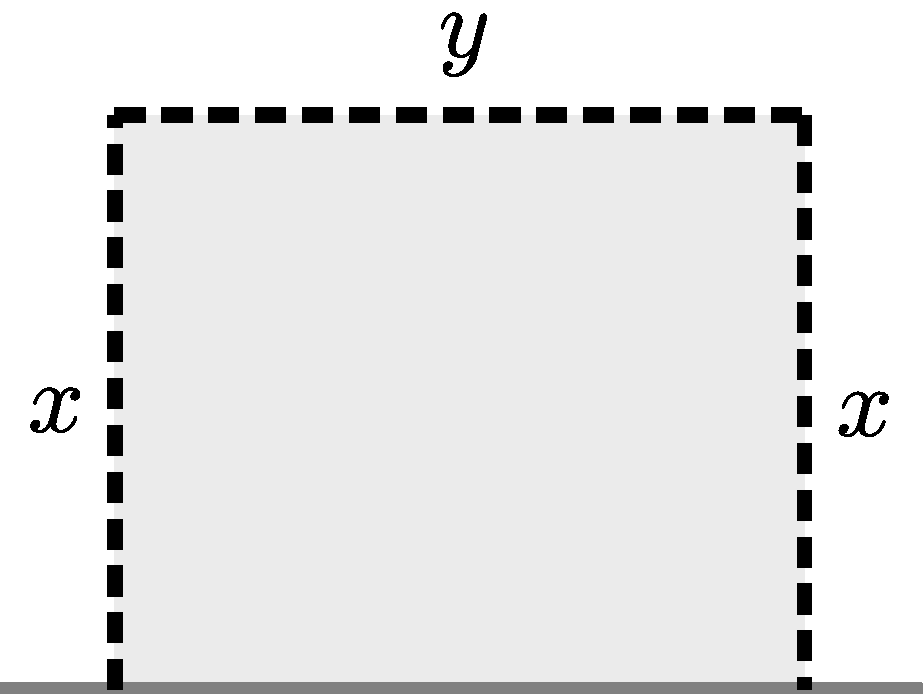
\includegraphics[width=0.9\textwidth]{images/fence}
\end{minipage}
\end{exercise}
\begin{comment}
\begin{solution*}
	\phantom{text}
	\begin{tasks}
		\task The enclosure wants to ``use'' as much of the wall as it can.
		Thus we expect the edge parallel to the wall to be a bit larger than the the two edges orthogonal to the wall.
		\task $f(x)=x\cdot\left(64-2x\right)$
		\task Plug in $a=64$ below.
		\task The area of the garden is given by $x\cdot y$ with the \textbf{constraint} $2x+y=a$.
		We use the constraint to replace $y$.
		Thereby we obtain the target function
		\begin{equation*}
			f\left(x\right)=x\cdot\left(a-2x\right)
		\end{equation*}
		for the surrounded area.
		If we set the derivative
		\begin{equation*}
			f^\prime\left(x\right)=-2x+\frac{a}{4}.
		\end{equation*}
		to zero and solve for $x$, we obtain $x_0=\frac{a}{4}$.
		This is indeed a maximum since
		\begin{equation*}
			f^{\prime\prime}\left(x\right)=-2
		\end{equation*}
		is negative at every $x$ and in particular at $x_0$.
	\end{tasks}
\end{solution*}
\end{comment}

\begin{minipage}{0.6\textwidth}
	\begin{exercise}
		We consider a piece of cardboard in the shape of a square.
		After cutting off small squares at each corner (see the figure
		to the right) the remaining cardboard can be folded to create
		a box with the top side open.
		\begin{tasks}
			\task Suppose the cardboard has side length 10 dm.
			For which side length x of the small squares will
			the volume $V(x)$ of the box be as large as possible?
			\task Generalize for the case that the cardboard has side
			length $a$.
		\end{tasks}
	\end{exercise}
\end{minipage}\hfill
\begin{minipage}{0.39\textwidth}
	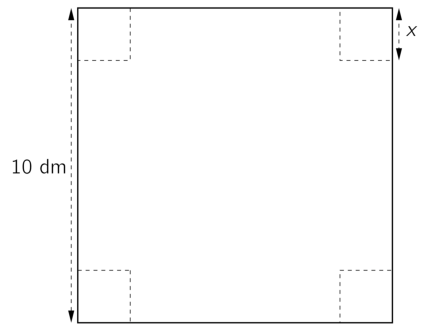
\includegraphics[width=\textwidth]{images/box}
\end{minipage}\\
\begin{comment}
	\begin{solution*}
		\phantom{text}
		\begin{tasks}
			\task The target function is
			\begin{equation*}
				f\left(x\right)=x\cdot\left(10-2x\right)^2
				=4x^3-40x^2+100x
			\end{equation*}
			with derivative
			\begin{equation*}
				f^{\prime}\left(x\right)=12x^2-80x+100.
			\end{equation*}
			The zeros of the derivative are given by
			\begin{equation*}
				\frac{1}{6}\cdot\left(20\pm\sqrt{400-4\cdot 3\cdot 25}\right)
				=\frac{1}{3}\left(10\pm 5\right).
			\end{equation*}
			Clearly, $x_0=5$ dm means an empty box.
			We thus proceed with $x_0=\frac{5}{3}$ dm.
			We have
			\begin{equation*}
				f^{\prime\prime}\left(x\right)=24x-80
			\end{equation*}
			and therefore $f^{\prime\prime}(\frac{5}{3})=-40$.
			We conclude that $x_0=\frac{5}{3}$ dm is a maximum.
			\task In a similar way, we find $x=\frac{a}{6}$.
		\end{tasks}
	\end{solution*}
\end{comment}

\begin{exercise}
	A sector of a circle has a perimeter (Umfang) $p$.
	Find the radius and central angle of the sector
	which will maximize its area.
\end{exercise}
\begin{comment}
	\begin{solution*}
		Let $r$ be the radius and let $\alpha$ be the central angle in radians.
		The perimeter yields the constraint
		\begin{equation*}
			\alpha\cdot r+2r=p,
		\end{equation*}
		which yields is equivalent to $\alpha=\frac{p}{r}-2$.
		The area is given by
		\begin{equation*}
			A\left(r\right)=\frac{\alpha}{2\pi}\cdot \pi r^2
			=-r^2+\frac{p}{2}\cdot r,
		\end{equation*}
		where we have substituted $\alpha$ in the last step.
		The first derivative
		\begin{equation*}
			A^{\prime}\left(r\right)=-2r+\frac{p}{2}
		\end{equation*}
		yields the critical point $r_0=\frac{p}{4}$.
		This is a maximum since
		\begin{equation*}
			A^{\prime\prime}\left(r\right)=-2
		\end{equation*}
		is negative for every radius and in particular for $r_0$.
		The corresponding angle is given by
		\begin{equation*}
			\alpha_0=\frac{p}{r_0}-2=2.
		\end{equation*}
		This corresponds to $\alpha_0\cdot\frac{360}{2\pi}\approx 114.6$ degrees.
	\end{solution*}
\end{comment}

\begin{minipage}{0.8\textwidth}
	\begin{exercise}
		We want to build a window with a semicircle on top (see image).
		If there is 12 meters of framing materials,
		what must be the dimensions of the window to let in the most light
		(i.e. maximal area)?
	\end{exercise}
\end{minipage}\hfill
\begin{minipage}{0.15\textwidth}
	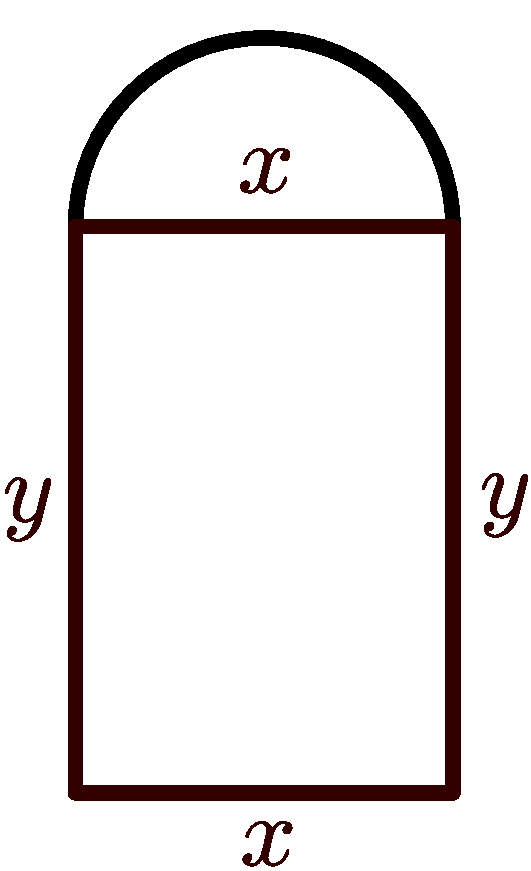
\includegraphics[width=\textwidth]{images/window}
\end{minipage}\\
\begin{comment}
\begin{solution*}
	The formulas for the perimeter (Umfang) and the area are given by
	\begin{equation*}
		\left(1+\frac{\pi}{2}\right)x+2y
		\quad\text{and}\quad
		\frac{\pi}{8}x^2+xy,
	\end{equation*}
	respectively.
	Since the perimeter equals 12 meters, we set the first equation equal to 12 and solve for $y$.
	We obtain
	\begin{equation*}
		y=-\frac{\pi+2}{4}x^2+6
	\end{equation*}
	and plug this into the equation for the area, which becomes our target function
	\begin{equation*}
		f\left(x\right)=-\frac{\pi+4}{8}x^2+6x.
	\end{equation*}
	To find the critical point(s), we set the derivative
	\begin{equation*}
		f^{\prime}\left(x\right)=-\frac{\pi+4}{4}x+6
	\end{equation*}
	equal to zero and solve for $x$.
	We get
	\begin{equation*}
		x_0=\frac{24}{\pi+4}.
	\end{equation*}
	This is indeed a maximum, since
	\begin{equation*}
		f^{\prime\prime}\left(x\right)=-\frac{\pi+4}{4}
	\end{equation*}
	is negative at every $x$ and in particular at $x_0$.
\end{solution*}
\end{comment}

\begin{minipage}{0.7\textwidth}
\begin{exercise}
	\textcolor{gray}{(hard)} In a triangle, we are given the altitude $h$ and the corresponding base line $b$.
	What are the side length of an inscribed rectangle of maximal area?
\end{exercise}
\end{minipage}\hfill
\begin{minipage}{0.25\textwidth}
	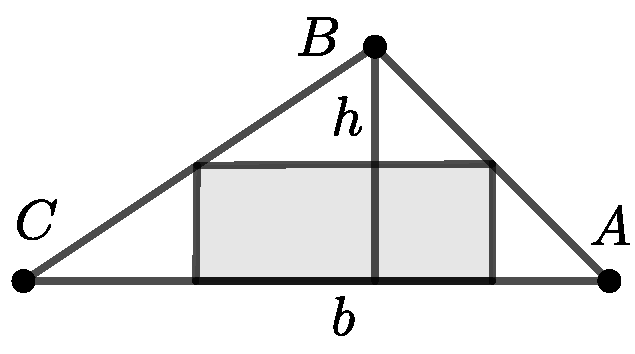
\includegraphics[width=\textwidth]{images/triangle}
\end{minipage}\\
\end{document}